\documentclass[aspectratio=169, usenames, dvipsnames]{beamer}

\usetheme{Pittsburgh}

\usepackage[utf8]{inputenc}
\usepackage{amsmath}
\usepackage{amsfonts}
\usepackage{amssymb}
\usepackage{graphicx}
\usepackage{multicol}
\usepackage{hyperref}
\usepackage{framed}
\usepackage{tikz}
\usetikzlibrary{shapes,arrows,positioning}
\usepackage{xspace}                     % Correct spacings
\usepackage{csquotes} 
\usepackage{stex-logo}
\usepackage{lmodern}

\usepackage{tkz-kiviat}

\beamertemplatenavigationsymbolsempty 
\setbeamertemplate{footline}[frame number]

\newcommand{\MMT}{\textsf{MMT}\xspace}
\newcommand{\OMDOC}{\textsf{OMDoc}\xspace}
\def\ALeA{\textsc{ALeA}\xspace}

\author{Jonas Betzendahl and Michael Kohlhase and Dennis Müller}
\title{Guided Tours in \ALeA}
\subtitle{Assembling Tailored Educational Dialogues from Semantically Annotated Learning Objects}

\begin{document}

%------------------------------------------------------------------------------------
\begin{frame}
\begin{center}
\huge \textbf{Guided Tours in \ALeA}\medskip

\large Assembling Tailored Educational Dialogues\\ from Semantically Annotated Learning Objects

\normalsize 
\bigskip\bigskip

\large \emph{Jonas Betzendahl}, Michael Kohlhase, Dennis Müller\\
\texttt{[firstname].[lastname]@fau.de}\bigskip

\small
AI4AI Workshop @ ECAI23\\
2023 -- 09 -- 30
\bigskip

\includegraphics[scale=0.5]{images/fau_logo.png}
\quad
\includegraphics[scale=0.25]{images/kwarclogo_faublau.png} 
\quad
\includegraphics[scale=0.18]{images/voll-ki} 
\end{center}
\end{frame}

\section{Introduction}

\begin{frame}
\frametitle{Motivation}
\begin{minipage}{0.55\textwidth}
Education is becoming more diverse in terms of neurotypes, cultural and educational backgrounds as well as educational goals and more.
\bigskip

\Large This is a good thing!
\bigskip

\normalsize However, due to staffing and budget constraints, not all institutions can compensate. The shift to online delivery of course materials often does not address this.
\end{minipage}
\hfill
\begin{minipage}{0.4\textwidth}
\includegraphics[height=0.6\textheight,keepaspectratio]{images/group_session} 
\end{minipage}%
\end{frame}

\begin{frame}[fragile]
\frametitle{Context: \ALeA}

In \ALeA, our learning-platform-shaped answer to these problems\footnote{For details, please see: \url{https://url.mathhub.info/CICM23ALEA/}}, we contend that any good educator (human or not) relies on four different models for teaching:
\bigskip

\begin{minipage}{0.4\textwidth}
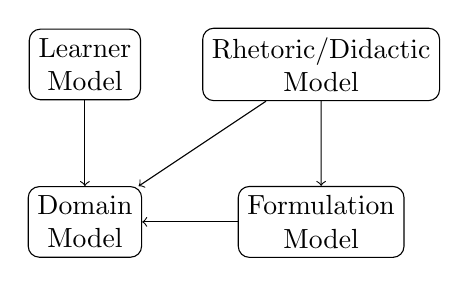
\begin{tikzpicture}[xscale=3,yscale=2]
  \node[draw,rounded corners,align=center] (dm) at (0,0) {Domain\\ Model};
  \node[draw,rounded corners,align=center] (lm) at (0,1) {Learner\\ Model};
  \node[draw,rounded corners,align=center] (fm) at (1,0) {Formulation\\ Model};
  \node[draw,rounded corners,align=center] (im) at (1,1) {Rhetoric/Didactic\\ Model};
  \draw[->] (lm) -- (dm);
  \draw[->] (fm) -- (dm);
  \draw[->] (im) -- (dm);
  \draw[->] (im) -- (fm);
\end{tikzpicture}
\end{minipage}%
\begin{minipage}{0.6\textwidth}
\begin{itemize}
\pause
\item Domain Model\\
\emph{Information about concepts and their relations}
\pause
\item Formulation Model\\
\emph{Learning objects of all varieties}
\pause
\item Rhetoric Model\\
\emph{Didactic classification of learning objects}
\pause
\item Learner Model\\
\emph{Estimation of educatee competency distribution}
\end{itemize}
\end{minipage}%
\end{frame}

\begin{frame}
\frametitle{\sTeX}
\begin{center}
How we do it: Semantic annotation on the \emph{concept level} in course materials.\bigskip

\includegraphics[width=0.95\textwidth, keepaspectratio]{images/stex_example.png} 
\end{center}
\end{frame}

\begin{frame}[fragile]
\frametitle{The Learner Model}
\begin{minipage}{0.4\textwidth}
Our learner model uses a revised version of Bloom's taxonomy of educational objectives. It tracks six cognitive dimensions for every student for every concept they have encountered.
\bigskip

The model is under full control of the learners and can be primed by them on initialisation with their educational history.
\end{minipage}%
\hfill
\begin{minipage}{0.55\textwidth}
\begin{tikzpicture}[rotate=-35, scale=0.5]
\tkzKiviatDiagram[label space = 1.5]{Remember,Understand,Apply,Analyse,Evaluate,Create}
\tkzKiviatLine[thick,color=red](7.25,5.5,4,6.5,7,2)
\pause
\tkzKiviatLine[thick,color=blue](3,9,6,5.2,5.6,4.8)
\pause
\tkzKiviatLine[thick,color=ForestGreen](5.9,6.1,3,3,2.3,9.2)
\end{tikzpicture}
\end{minipage}%
\end{frame}

\section{The Algorithm}

\begin{frame}
\frametitle{Educational Dialogues}
\begin{minipage}{0.45\textwidth}
This granular and precise learner model allows us to offer \emph{tailored}
educational services that take into account the knowledge state of the individual.
\bigskip

One such service are \emph{guided tours}, mini-courses assembled on the fly, that students can request for any topic. They begin at precisely their current knowledge level and step-by-step work up to the concept they wanted to understand. This is presented in dialogue form to mimic one-on-one tutoring.
\end{minipage}%
\hfill
\begin{minipage}{0.5\textwidth}
\pause
\includegraphics[height=0.75\textheight,keepaspectratio]{images/bubbles_example_step1} 
\end{minipage}%
\end{frame}

\begin{frame}
\frametitle{Educational Dialogues}
\begin{minipage}{0.45\textwidth}
This granular and precise learner model allows us to offer \emph{tailored}
educational services that take into account the knowledge state of the individual.
\bigskip

One such service are \emph{guided tours}, mini-courses assembled on the fly, that students can request for any topic. They begin at precisely their current knowledge level and step-by-step work up to the concept they wanted to understand. This is presented in dialogue form to mimic one-on-one tutoring.
\end{minipage}%
\hfill
\begin{minipage}{0.5\textwidth}
\includegraphics[height=0.75\textheight,keepaspectratio]{images/bubbles_example_step2} 
\end{minipage}%
\end{frame}

\begin{frame}
\frametitle{Educational Dialogues}
\begin{minipage}{0.45\textwidth}
This granular and precise learner model allows us to offer \emph{tailored}
educational services that take into account the knowledge state of the individual.
\bigskip

One such service are \emph{guided tours}, mini-courses assembled on the fly, that students can request for any topic. They begin at precisely their current knowledge level and step-by-step work up to the concept they wanted to understand. This is presented in dialogue form to mimic one-on-one tutoring.
\end{minipage}%
\hfill
\begin{minipage}{0.5\textwidth}
\includegraphics[height=0.75\textheight,keepaspectratio]{images/bubbles_example_step3} 
\end{minipage}%
\end{frame}

\begin{frame}
\frametitle{Educational Dialogues}
\begin{minipage}{0.45\textwidth}
This granular and precise learner model allows us to offer \emph{tailored}
educational services that take into account the knowledge state of the individual.
\bigskip

One such service are \emph{guided tours}, mini-courses assembled on the fly, that students can request for any topic. They begin at precisely their current knowledge level and step-by-step work up to the concept they wanted to understand. This is presented in dialogue form to mimic one-on-one tutoring.
\end{minipage}%
\hfill
\begin{minipage}{0.5\textwidth}
\includegraphics[height=0.75\textheight,keepaspectratio]{images/bubbles_example_step4} 
\end{minipage}%
\end{frame}

\begin{frame}
\frametitle{Educational Dialogues}
\begin{minipage}{0.45\textwidth}
This granular and precise learner model allows us to offer \emph{tailored}
educational services that take into account the knowledge state of the individual.
\bigskip

One such service are \emph{guided tours}, mini-courses assembled on the fly, that students can request for any topic. They begin at precisely their current knowledge level and step-by-step work up to the concept they wanted to understand. This is presented in dialogue form to mimic one-on-one tutoring.
\end{minipage}%
\hfill
\begin{minipage}{0.5\textwidth}
\includegraphics[height=0.75\textheight,keepaspectratio]{images/bubbles_example_step5} 
\end{minipage}%
\end{frame}

\begin{frame}
\frametitle{Overview}
\begin{minipage}{0.7\textwidth}
\vspace*{-10px}
\includegraphics[height=0.9\textheight,keepaspectratio]{images/gt_algorithm_square}
\end{minipage}%
\begin{minipage}{0.3\textwidth}
The complete algorithm for guided tours in \ALeA.
\end{minipage}%
\end{frame}

\begin{frame}
\frametitle{Initialisation}
\begin{minipage}{0.7\textwidth}
\vspace*{-10px}
\includegraphics[height=0.9\textheight,keepaspectratio]{images/gt_algorithm_square_step1}
\end{minipage}%
\begin{minipage}{0.3\textwidth}
Important points:
\bigskip
\begin{itemize}
\item Assemble the dependency graph of domain concepts\\
\item No trivial guided tours allowed
\end{itemize}
\end{minipage}%
\end{frame}

\begin{frame}
\frametitle{Aside: cut-off points}
\begin{minipage}{0.5\textwidth}
\begin{center}
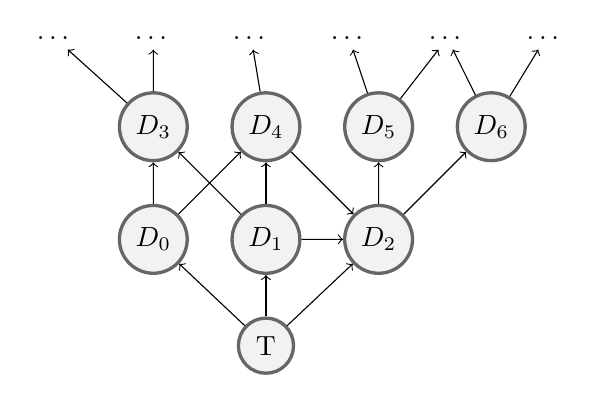
\begin{tikzpicture}[xscale=0.75,yscale=0.75,node distance=15pt, roundnode/.style={circle, draw=black!60, fill=black!5, very thick, minimum size=7mm}]
%Nodes
\node[roundnode]      (target) {T};
\node[roundnode]      (d1)       [above=of target] {$D_1$};
\node[roundnode]      (d0)       [left=of d1] {$D_0$};
\node[roundnode]      (d2)       [right=of d1] {$D_2$};
\node[roundnode]      (d3)       [above=of d0] {$D_3$};
\node[roundnode]      (d4)       [above=of d1] {$D_4$};
\node[roundnode]      (d5)       [above=of d2] {$D_5$};
\node[roundnode]      (d6)       [right=of d5] {$D_6$};
\node (inf1) [above=of d3] {\dots};
\node (inf0) [left=of inf1] {\dots};
\node (inf2) [right=of inf1] {\dots};
\node (inf3) [right=of inf2] {\dots};
\node (inf4) [right=of inf3] {\dots};
\node (inf5) [right=of inf4] {\dots};

\draw[->] (target) -- (d0);
\draw[->] (target) -- (d1);
\draw[->] (target) -- (d2);
\draw[->] (d0) -- (d3);
\draw[->] (d0) -- (d4);
\draw[->] (d1) -- (d3);
\draw[->] (d1) -- (d4);
\draw[->] (d2) -- (d5);
\draw[->] (d2) -- (d6);
\draw[->] (d4) -- (d2);
\draw[->] (d1) -- (d2);

\draw[->] (d6) -- (inf4);
\draw[->] (d6) -- (inf5);
\draw[->] (d5) -- (inf4);
\draw[->] (d5) -- (inf3);
\draw[->] (d3) -- (inf0);
\draw[->] (d3) -- (inf1);
\draw[->] (d4) -- (inf2);
\end{tikzpicture}
\end{center}
\end{minipage}%
\hfill
\begin{minipage}{0.45\textwidth}
When we talk about \emph{cut-off points}, we mean any concept in the dependency closure of our target that the educatee already understands ``sufficiently''.
\bigskip

We do not present them \emph{or any of only their dependencies} to the learner, even if their dependencies are not yet ``sufficiently'' understood.
\end{minipage}%
\end{frame}

\begin{frame}
\frametitle{Concept Introduction}
\begin{minipage}{0.7\textwidth}
\vspace*{-10px}
\includegraphics[height=0.9\textheight,keepaspectratio]{images/gt_algorithm_square_step2}
\end{minipage}%
\begin{minipage}{0.3\textwidth}
Important points:
\bigskip
\begin{itemize}
\item Always present familiar definition\\
\item Cooldown to avoid LO doubling
\end{itemize}
\end{minipage}%
\end{frame}

\begin{frame}
\frametitle{Learning}
\begin{minipage}{0.7\textwidth}
\vspace*{-10px}
\includegraphics[height=0.9\textheight,keepaspectratio]{images/gt_algorithm_square_step3}
\end{minipage}%
\begin{minipage}{0.3\textwidth}
Important points:
\bigskip
\begin{itemize}
\item ``Most Helpful'' LO varies by context\\
\item Updates to learner model can change graph.
\end{itemize}
\end{minipage}%
\end{frame}

\begin{frame}
\frametitle{Finish}
\begin{minipage}{0.7\textwidth}
\vspace*{-10px}
\includegraphics[height=0.9\textheight,keepaspectratio]{images/gt_algorithm_square_step4}
\end{minipage}%
\begin{minipage}{0.3\textwidth}
When all relevant concepts in the dependency hull have been mastered, the guided tour concludes.
\end{minipage}%
\end{frame}

\section{Wrap-up}

\begin{frame}
\frametitle{Summary}
\begin{minipage}{0.7\textwidth}
\vspace*{-10px}
\includegraphics[height=0.9\textheight,keepaspectratio]{images/gt_algorithm_square}
\end{minipage}%
\begin{minipage}{0.3\textwidth}
Diverse educational backgrounds demand solutions tailored to the individual.\bigskip

Semantic annotations of course materials using \sTeX allow for granular learner models.\bigskip

Guided tours in \ALeA are educational dialogues that are assembled for where the student is and where they want to go.
\end{minipage}%
\end{frame}

\end{document}